\documentclass[aspectratio=169,xcolor=table]{beamer}
\usepackage[utf8]{inputenc}
\usepackage[T1,T5]{fontenc}
\usepackage{amsmath,amssymb,booktabs,array,graphicx,tikz}
\usetikzlibrary{positioning,arrows.meta}

\definecolor{Primary}{HTML}{111B88}
\definecolor{Secondary}{HTML}{101659}
\definecolor{Accent}{HTML}{F2A900}
\definecolor{SoftBlue}{HTML}{EAF2F8}
\definecolor{TextGray}{HTML}{4D5966}
\definecolor{RiskRed}{HTML}{A23B3B}
\definecolor{GoodGreen}{HTML}{26734D}
\mode<presentation>{\usetheme{Madrid}\usecolortheme{default}\setbeamertemplate{navigation symbols}{}}
\setbeamercolor{structure}{fg=Primary}
\setbeamercolor{frametitle}{fg=white,bg=Primary}
\setbeamercolor{title}{fg=white,bg=Primary}
\setbeamercolor{block body}{fg=black,bg=SoftBlue}
\setbeamercolor{block body alerted}{fg=black,bg=Accent!12}
\setbeamercolor{section in head/foot}{fg=white,bg=Primary}
\setbeamercolor{author in head/foot}{fg=white,bg=Secondary}
\setbeamercolor{date in head/foot}{fg=white,bg=Primary}
\setbeamerfont{section in head/foot}{size=\tiny,series=\bfseries}
\setbeamerfont{author in head/foot}{size=\scriptsize}
\setbeamerfont{date in head/foot}{size=\scriptsize,series=\bfseries}
\setbeamerfont{frametitle}{series=\bfseries}
\setbeamerfont{title}{series=\bfseries}
\newcommand{\decklabel}{Contextual ASR -- Scorer}
\setbeamertemplate{itemize item}{\color{Secondary}$\blacktriangleright$}
\setbeamertemplate{itemize subitem}{\color{Accent}$\bullet$}
\setbeamertemplate{headline}{\leavevmode\begin{beamercolorbox}[wd=\paperwidth,ht=2.7ex,dp=1.1ex,leftskip=.35cm,rightskip=.35cm]{section in head/foot}\insertsectionnavigationhorizontal{\dimexpr\paperwidth-.70cm\relax}{}{}\end{beamercolorbox}}
\setbeamertemplate{footline}{\leavevmode\hbox{\begin{beamercolorbox}[wd=.55\paperwidth,ht=2.6ex,dp=1ex,leftskip=.35cm,rightskip=.20cm]{section in head/foot}\usebeamerfont{section in head/foot}\insertsectionhead\end{beamercolorbox}\begin{beamercolorbox}[wd=.27\paperwidth,ht=2.6ex,dp=1ex,center]{author in head/foot}\usebeamerfont{author in head/foot}\decklabel\end{beamercolorbox}\begin{beamercolorbox}[wd=.18\paperwidth,ht=2.6ex,dp=1ex,rightskip=.35cm plus1fil]{date in head/foot}\usebeamerfont{date in head/foot}\hfill\insertframenumber\,/\,\inserttotalframenumber\end{beamercolorbox}}}
\newcolumntype{L}[1]{>{\raggedright\arraybackslash}p{#1}}
\newcommand{\hi}[1]{\textcolor{Primary}{\textbf{#1}}}
\newcommand{\bad}[1]{\textcolor{RiskRed}{\textbf{#1}}}
\newcommand{\good}[1]{\textcolor{GoodGreen}{\textbf{#1}}}
\newcommand{\src}[1]{{\tiny\color{TextGray}[#1]}}
\newcommand{\ra}{$\rightarrow$}
\newcommand{\nbox}[2][block body]{\begin{beamercolorbox}[sep=0.45em,rounded=true]{#1}\footnotesize #2\end{beamercolorbox}}

\title{Scorer: số liệu, thí nghiệm, và cách dùng vị trí của từ}
\subtitle{Kết quả hiện tại \ra{} việc còn lại \ra{} chọn SpeechLLM \ra{} kế hoạch tới Interspeech 2027}
\author{Nhóm Contextual ASR}
\institute{}
\date{11/2026}
\setbeamertemplate{title page}{\begin{centering}\vspace*{0.10cm}
\includegraphics[height=1.08cm]{../2026-10-23/imgs/logo.png}\par\vspace{0.32cm}\begin{beamercolorbox}[sep=0.50em,center,rounded=true]{title}\usebeamerfont{title}\inserttitle\par\vspace{0.14cm}{\small\insertsubtitle\par}\end{beamercolorbox}\vspace{0.42cm}{\usebeamerfont{author}\insertauthor\par}\vspace{0.10cm}{\usebeamerfont{institute}\insertinstitute\par}\vfill{\usebeamerfont{date}\insertdate\par}\end{centering}}

\begin{document}
\begin{frame}[plain]\titlepage\end{frame}

% ------------------------------------------------------------------
\section{Tóm tắt}
\begin{frame}{Buổi này em báo cáo 3 ý}
\nbox{\textbf{\textcircled{\scriptsize 1} Scorer:} dùng được (97.7\% từ đúng vào prompt, test-other N2000) nhưng \bad{chưa chứng minh là kiến trúc tốt nhất}: chưa chạy âm vị--âm vị thật. \bad{Đính chính buổi trước:} ``thắng Hou25 8/8 ô'' chỉ đúng khi so với \textbf{số trong paper}; cùng pipeline với bản tái hiện của Hoàng thì pxattn \bad{kém 0.2--0.9} B-WER.}
\vspace{0.12cm}
\nbox{\textbf{\textcircled{\scriptsize 2} Vị trí:} scorer \good{tự biết từ nằm ở đâu} mà không cần giám sát: attention lớp 1 sai số 0.03 s, căn tới mức âm vị. Không cần TTS.}
\vspace{0.12cm}
\nbox[block body alerted]{\textbf{\textcircled{\scriptsize 3} Đi tiếp:} lỗi lớn nhất còn lại là \hi{nghe giống}: ngay cả với list oracle vẫn còn 2.33 / 4.62 điểm, nên đổi list hay đổi prompt không chạm tới được. Đề xuất: chạy \hi{S0 (âm vị--âm vị)} rồi mới chốt scorer, sau đó \hi{can thiệp logit lúc decode, dùng p và thời gian làm cổng} để không chèn từ sai (\bad{ý tưởng, chưa chạy}). }
\vspace{0.12cm}
{\footnotesize Mỗi ô số: test-clean / test-other. B-WER = lỗi trên từ hiếm, thấp là tốt. Whisper dùng chuẩn hoá plain, Qwen dùng wnorm.}
\end{frame}

\begin{frame}{Đang làm gì: scorer nghe audio, độc lập với mô hình ASR}
\centering
\begin{tikzpicture}[font=\footnotesize,>={Stealth},
  box/.style={draw=Primary,fill=SoftBlue,rounded corners=2pt,minimum height=0.85cm,align=center,inner sep=4pt},
  new/.style={draw=Accent,fill=Accent!15,rounded corners=2pt,minimum height=0.85cm,align=center,inner sep=4pt}]
\node[box,minimum width=1.9cm] (a) at (0,0) {audio};
\node[box,minimum width=1.9cm] (l) at (0,-1.7) {list\\2000 từ};
\node[box,minimum width=2.7cm] (s) at (3.6,-1.7) {\textbf{scorer}\\(âm vị + attention)};
\node[box,minimum width=3.0cm] (asr) at (10.6,0) {\textbf{SpeechLLM}\\Whisper, Qwen3-ASR, \ldots};
\node[box,minimum width=1.5cm] (t) at (13.5,0) {text};
\node[box,minimum width=2.6cm] (p) at (7.4,-1.7) {từ được chọn\\top-50 hoặc $p\geq\theta$};
\node[new,minimum width=2.6cm] (g) at (7.4,-3.1) {(từ, $p$, $t_{\text{đầu}}$, $t_{\text{cuối}}$)};
\draw[->,thick] (a) -- (asr);
\draw[->,thick] (asr) -- (t);
\draw[->,thick] (l) -- (s);
\draw[->,thick] (a.south east) -- (s.north west);
\draw[->,thick] (s) -- (p);
\draw[->,thick] (p.east) -| node[pos=0.72,right,font=\scriptsize,align=left]{đã làm:\\prompt} (asr.south);
\draw[->,thick] (s.south) |- (g.west);
\draw[->,thick,Accent!90!black] (g.east) -| node[pos=0.25,below,font=\scriptsize,text=black]{bước tiếp: cổng lúc decode} (asr.south east);
\end{tikzpicture}
\par\vspace{0.3cm}\raggedright
\nbox{\textbf{Bài toán:} list càng dài và nhiều nhiễu thì SpeechLLM càng bỏ sót từ đúng, và càng tự chèn từ trong list dù audio không có. \textbf{Benchmark:} LibriSpeech test-clean (2620 câu) / test-other (2939 câu) + list IS21, N từ 100 tới 2000.}
\end{frame}

% ------------------------------------------------------------------
\section{Số liệu}
\begin{frame}{Scorer pxattn khác Hou25 ở đâu}
\centering\scriptsize\setlength{\tabcolsep}{4pt}
\begin{tabular}{L{1.8cm}L{3.5cm}L{3.5cm}L{5.1cm}}
\toprule
 & Hou25 \src{paper §2.2} & pxattn (nhóm) & Lý do thiết kế \\
\midrule
Biểu diễn từ & audio TTS qua encoder Whisper & \hi{âm vị g2p} + 2 lớp Transformer & không cần TTS; từ mới chấm được ngay; phía từ không có ``giọng'' \\
Phía audio & Whisper đóng băng + Linear & Whisper đóng băng + Linear + 1 lớp Transformer & giữ nguyên encoder để chỉ đổi cách biểu diễn từ \\
So khớp & 4 ma trận cosine \ra{} CNN & âm vị là query, cross-attention 2 lớp & âm vị không có thời lượng, không có vệt chéo cho CNN bắt \\
Gộp & average pool & [mean; max] theo âm vị & max giữ được một khớp ngắn trong câu dài \\
Đầu ra & softmax ra điểm & \hi{sigmoid, BCE từng cặp} & xác suất độc lập: lọc được theo ngưỡng, list được phép rỗng \\
Tốc độ & 922 ms/câu & \good{332 ms/câu} (N2000) & \\
\bottomrule
\end{tabular}\par
\vspace{0.25cm}\raggedright
\nbox{Train cùng dữ liệu với Hou25: train-clean-100. pxattn có 4.96M tham số. Biến thể rẻ hơn là pmaxsim (mỗi âm vị lấy frame giống nhất): phía từ tính trước được cho cả kho.}
\end{frame}

\begin{frame}{Bảng A -- B-WER trên Whisper-turbo, top-50, prompt naive}
\centering\footnotesize\setlength{\tabcolsep}{4pt}
\begin{tabular}{llcccc}
\toprule
 & & N=100 & N=500 & N=1000 & N=2000\\
\midrule
Mốc & không prompt & 9.43 / 18.92 & $\leftarrow$ & $\leftarrow$ & $\leftarrow$\\
 & nguyên list & 8.04 / 13.98 & 8.87 / 18.22 & 9.20 / 18.32 & 9.15 / 18.69\\
 & Hou25 \src{số paper} & 5.4 / 10.0 & 5.4 / 10.7 & 5.6 / 11.3 & 5.8 / 11.7\\
\midrule
Pipeline nhóm & pxattn & \textbf{4.57 / 8.92} & \textbf{4.89 / 9.21} & \textbf{5.16 / 9.79} & \textbf{5.29 / 10.00}\\
 & pmaxsim & 4.60 / 10.30 & 4.95 / 9.53 & 5.17 / 9.83 & 5.47 / 10.37\\
\midrule
Pipeline Hoàng & Hou25 tái hiện & \good{4.4 / 8.7} & \good{4.5 / 8.8} & \good{4.6 / 9.5} & \good{4.9 / 9.2}\\
\src{mlx-whisper} & pxattn & 4.6 / 9.0 & 4.8 / 9.3 & 5.1 / 9.9 & 5.1 / 10.1\\
\bottomrule
\end{tabular}\par
\vspace{0.2cm}\raggedright
\begin{columns}[T]
\begin{column}{0.48\textwidth}
\nbox{\textbf{Đọc:} scorer giảm B-WER khoảng một nửa so với nguyên list ở N lớn. Nguyên list N$\geq$1000 bị cắt còn 223 token, chỉ 2--6\% từ đúng còn lại trong prompt.}
\end{column}
\begin{column}{0.48\textwidth}
\nbox[block body alerted]{\textbf{Nói thẳng:} so công bằng là 2 hàng cuối, cùng pipeline: pxattn \bad{kém 0.2--0.9}. Hiện 1 seed, chưa có khoảng tin cậy; \textbf{cần file hyp từng câu của Hoàng}.}
\end{column}
\end{columns}
\end{frame}

\begin{frame}{Bảng B -- Qwen3-ASR-1.7B, list N2000: lọc ngưỡng là tốt nhất}
\begin{columns}[T]
\begin{column}{0.58\textwidth}
\centering\footnotesize\setlength{\tabcolsep}{4pt}
\begin{tabular}{lcc}
\toprule
 & WER & B-WER\\
\midrule
không context & 1.63 / 3.41 & 7.40 / 16.08\\
nguyên list N2000 & 1.69 / 3.55 & 7.40 / 16.45\\
pxattn top-50 & 1.47 / 2.95 & 5.71 / 11.57\\
\textbf{pxattn lọc $p\geq0.5$} & \good{1.32 / 2.68} & \good{4.78 / 9.71}\\
oracle (chỉ từ đúng) & 1.22 / 2.43 & 4.01 / 7.73\\
\midrule
\texttt{missing\_N2000} \ra{} $p\geq0.5$ & 1.65 / 3.42 & 7.39 / 16.18\\
\bottomrule
\end{tabular}\par
\vspace{0.15cm}\raggedright
{\scriptsize\color{TextGray} Tham chiếu PTC-Bias \src{arXiv 2609.28727}, trên Qwen3-ASR-\textbf{0.6B} nên không so trực tiếp: CTC-Filter 4.81 / 9.45; PTC 4.10 / 7.76.}
\end{column}
\begin{column}{0.40\textwidth}
\nbox{\textbf{Lọc ngưỡng:} xác suất của scorer dùng được thật, đưa Qwen tới gần oracle.}
\vspace{0.12cm}
\nbox{\textbf{List toàn nhiễu} (\texttt{missing}): scorer đưa Qwen về đúng mức không context (7.39 so với 7.40), tức list nhiễu không còn kéo sai.}
\vspace{0.12cm}
\nbox[block body alerted]{Lưới đầy đủ trên Qwen (N100--2000) \bad{chưa chạy}: mới có N2000.}
\end{column}
\end{columns}
\end{frame}

\begin{frame}{Bảng C -- Chọn từ: tìm tốt, nhưng dễ bị từ nghe giống lừa}
\centering\footnotesize\setlength{\tabcolsep}{6pt}
\begin{tabular}{lccc}
\toprule
test-other, N2000 & R\_B\#50 $\uparrow$ & R\_B@99 $\downarrow$ & R\_H\#50 $\downarrow$\\
 & {\scriptsize từ đúng lọt top-50} & {\scriptsize số từ cần để giữ 99\% từ đúng} & {\scriptsize từ nghe giống lọt top-50}\\
\midrule
Hou25 tái hiện (Hoàng) & 97.43 & 256.4 & \good{17.26}\\
pxattn 100 h & 97.71 & 106.7 & \bad{21.58}\\
pmaxsim 100 h & 98.44 & 99.8 & \bad{25.52}\\
pxattn 960 h & \good{98.59} & \good{63.9} & \bad{21.47}\\
PTC-Bias \src{paper} & 99.30 & 16.9 & 22.00\\
\bottomrule
\end{tabular}\par
\vspace{0.3cm}\raggedright
\begin{columns}[T]
\begin{column}{0.48\textwidth}
\nbox{\textbf{Mạnh:} tìm từ đúng ngang hoặc hơn Hou25; ngưỡng hiệu chỉnh tốt hơn nhiều (@99: 107 so với 256).}
\end{column}
\begin{column}{0.48\textwidth}
\nbox[block body alerted]{\textbf{Yếu:} R\_H\#50 cao hơn Hou25 4--8 điểm. Mọi scorer đều còn thua PTC về @99.}
\end{column}
\end{columns}
\end{frame}

\begin{frame}{Bảng D -- Khoảng tin cậy ghép cặp (mới chạy, Whisper)}
\centering\small\setlength{\tabcolsep}{6pt}
\begin{tabular}{lcc}
\toprule
$\Delta$B-WER = A $-$ B \src{95\% CI, bootstrap theo câu, 1.000 lần} & clean & other\\
\midrule
pxattn N100 $-$ nguyên list N100 & \good{$-$3.47} [$-$6.16; $-$1.90] & \good{$-$5.07} [$-$5.78; $-$4.42]\\
pxattn N2000 $-$ nguyên list N2000 & \good{$-$3.85} [$-$4.46; $-$3.26] & \good{$-$8.69} [$-$9.63; $-$7.78]\\
\midrule
pxattn N100 $-$ pmaxsim N100 & $-$0.03 [$-$0.28; +0.21] & $-$1.38 [$-$5.57; +0.39]\\
pxattn N2000 $-$ pmaxsim N2000 & $-$0.17 [$-$0.53; +0.17] & $-$0.37 [$-$0.89; +0.14]\\
\midrule
pxattn $-$ Hou25 (Hoàng) & \bad{chưa có} & \bad{chưa có}\\
\bottomrule
\end{tabular}\par
\vspace{0.3cm}\raggedright
\nbox{\textbf{Đọc:} scorer hơn nguyên list là \good{có ý nghĩa thống kê} ở cả 4 ô. pxattn và pmaxsim \textbf{chưa phân biệt được} về B-WER (mọi khoảng đều chứa 0). Hiện ưu tiên pxattn vì \textbf{vị trí tới mức âm vị} và ít chèn nhiễu, không phải vì B-WER tốt hơn.}
\end{frame}

\begin{frame}{Vì sao âm vị? Chưa chứng minh được là tốt nhất}
\begin{columns}[T]
\begin{column}{0.60\textwidth}
\centering\scriptsize\setlength{\tabcolsep}{3pt}
\begin{tabular}{lcccc}
\toprule
test-other N2000, 1 seed & \#50 $\uparrow$ & @99 $\downarrow$ & H\#50 $\downarrow$ & chạy\\
\midrule
TTS $\leftrightarrow$ vector (Hou25, Hoàng) & 97.43 & 256.4 & \good{17.26} & thật\\
âm vị $\leftrightarrow$ vector (pxattn) & 97.71 & 106.7 & 21.58 & thật\\
âm vị $\leftrightarrow$ vector (pmaxsim) & 98.44 & 99.8 & 25.52 & thật\\
âm vị $\leftrightarrow$ chữ Qwen (hypmatch) & 95.41 & -- & 35.70 & thật\\
\textbf{âm vị $\leftrightarrow$ âm vị từ audio} (PTC) & \good{99.30} & \good{16.9} & 22.00 & \bad{số paper}\\
\bottomrule
\end{tabular}\par
\vspace{0.1cm}\raggedright
{\scriptsize\color{TextGray} PTC khác dữ liệu train; paper không ghi cách dựng tập từ nghe giống, nên chưa so công bằng.}\par
\vspace{0.15cm}
\nbox[block body alerted]{\textbf{Nói thẳng:} âm vị $\leftrightarrow$ âm vị thật \bad{chưa chạy}: hàng ``chữ Qwen'' không có model nhận dạng âm vị. Lý do đã chọn pxattn là không cần TTS, nhanh, chỉ đổi một biến so với Hou25; không phải đã thắng mọi cách.}
\end{column}
\begin{column}{0.36\textwidth}
\centering\scriptsize\setlength{\tabcolsep}{2pt}
\begin{tabular}{lc}
\toprule
Lựa chọn & đã kiểm?\\
\midrule
âm vị / TTS & có: đánh đổi\\
attention / max & có: ngang\\
hxattn, loss list & có: kém\\
2 lớp cross-attn & \bad{chưa}\\
lớp TF phía audio & \bad{chưa}\\
pool, 256 chiều & \bad{chưa}\\
\bottomrule
\end{tabular}\par
\vspace{0.2cm}\raggedright
\nbox{\ra{} \hi{Chưa chốt pxattn.} Chạy \textbf{S0} trước, xem trang kế hoạch.}
\end{column}
\end{columns}
\end{frame}

% ------------------------------------------------------------------
\section{Thí nghiệm + insight}
\begin{frame}{TN1 -- Đưa đúng từ mà Whisper vẫn có thể hỏng}
\begin{columns}[T]
\begin{column}{0.52\textwidth}
\centering\footnotesize\setlength{\tabcolsep}{3pt}
\begin{tabular}{lcc}
\toprule
N=100, cả tập & WER & B-WER\\
\midrule
không prompt & 2.64 / 4.87 & 9.43 / 18.92\\
\textbf{chỉ từ đúng (oracle)} & \bad{20.08 / 20.89} & 5.12 / \bad{26.24}\\
nguyên list, naive & 2.55 / 4.20 & 8.04 / 13.98\\
nguyên list, spoken & 2.32 / 4.30 & 7.12 / 14.56\\
pxattn top-50 & \good{2.18 / 3.66} & \good{4.57 / 8.92}\\
\bottomrule
\end{tabular}\par
\vspace{0.2cm}\raggedright
{\footnotesize Prompt chỉ 0--1 từ làm Whisper \textbf{lặp chữ}: khoảng 30 câu, mỗi câu thừa khoảng 430 từ. Câu có hơn 1 từ hiếm thì oracle bình thường: B-WER 4.33 / 8.63.}
\end{column}
\begin{column}{0.44\textwidth}
\nbox[block body alerted]{\textbf{Insight:} chọn từ hoàn hảo vẫn chưa đủ. \hi{Cách mô hình dùng list} là một nút thắt riêng, và phụ thuộc từng mô hình.}
\vspace{0.12cm}
\nbox{Qwen3-ASR không lặp chữ, nên $p\geq0.5$ dùng tốt. Trên Whisper dùng top-50, hoặc bọc câu spoken.}
\end{column}
\end{columns}
\end{frame}

\begin{frame}{TN2 -- Lỗi từ hiếm còn lại đến từ đâu (S1, mới)}
\centering\scriptsize\setlength{\tabcolsep}{3.5pt}
\begin{tabular}{lccccccccc}
\toprule
 & & \multicolumn{6}{c}{phần B-WER theo nguồn gốc} & & \\
\cmidrule(lr){3-8}
test-other & B-WER & xoá & ngoài & thay = & ranh & \textbf{nghe} & khác & chèn & nhiễu\\
 & & & prompt & nhiễu & giới & \textbf{giống} & & lặp & trong hyp\\
\midrule
không prompt & 18.92 & 0.86 & -- & -- & 1.53 & \textbf{10.24} & 6.28 & 0.00 & 0\\
oracle & 26.24 & 1.27 & -- & -- & 0.77 & \textbf{4.62} & 2.41 & \bad{17.18} & 0\\
pxattn N100 & 8.92 & 0.62 & 0.04 & 0.07 & 0.84 & \textbf{4.69} & 2.65 & 0.00 & 7\\
pxattn N2000 & 10.00 & 0.67 & \bad{1.68} & 0.34 & 0.65 & \textbf{4.32} & 2.34 & 0.00 & 54\\
pmaxsim N2000 & 10.37 & 0.79 & 1.23 & 0.39 & 0.73 & \textbf{4.47} & 2.77 & 0.00 & \bad{106}\\
\midrule
\bottomrule
\end{tabular}\par
\vspace{0.15cm}\raggedright
{\scriptsize test-clean: pxattn N2000 = 5.29 (ngoài prompt 0.54; thay = nhiễu 0.14; nghe giống 2.50); oracle nghe giống 2.33; nhiễu trong hyp: pxattn 13, pmaxsim 70.}\par
{\scriptsize\color{TextGray} Nghe giống = từ viết ra cách từ đúng $\leq$ 2 âm vị (g2p). Nhiễu trong hyp tính số lần, các cột khác tính điểm B-WER.}\par
\vspace{0.1cm}
\begin{columns}[T]
\begin{column}{0.48\textwidth}
\nbox{\textbf{Insight 1:} nghe giống ở pxattn \textbf{ngang oracle} (4.69 so với 4.62). Tầng prompt đã hết việc ở nhóm lỗi này: chỉ \hi{can thiệp lúc decode} mới chạm tới được.}
\end{column}
\begin{column}{0.48\textwidth}
\nbox[block body alerted]{\textbf{Insight 2:} từ nhiễu viết đè lên từ đúng chỉ tốn \bad{0.14 / 0.34} điểm, nên từ nghe giống trong prompt \textbf{chưa đủ giải thích} khoảng cách với Hou25.}
\end{column}
\end{columns}
\end{frame}

\begin{frame}{TN3 -- Scorer có biết từ nằm ở đâu không?}
\begin{columns}[T]
\begin{column}{0.56\textwidth}
\centering\scriptsize\setlength{\tabcolsep}{3pt}
\begin{tabular}{lccc}
\toprule
Bản đồ & sai số & trúng span & mức âm vị\\
\midrule
\textbf{pxattn attention lớp 1} & \good{0.03 / 0.03 s} & \good{99.5 / 99.2\%} & \good{có}\\
pmaxsim cosine & 0.04 / 0.03 s & 99.8 / 99.3\% & chỉ cả từ\\
Hou25 S1 & 0.06 / 0.06 s & 98.9 / 96.7\% & (frame TTS)\\
pxattn attention lớp 2 & -- & $\approx$ 50\% & không\\
pxattn cosine thô & -- & \bad{8.8 / 12.3\%} & không\\
\bottomrule
\end{tabular}\par
\vspace{0.1cm}\raggedright
{\scriptsize\color{TextGray} 400 câu/tập, mốc thời gian MFA (scorer không thấy lúc train). Mốc ngẫu nhiên 10.2 / 12.4\%.}\par
\vspace{0.15cm}
\nbox{\textbf{Insight:} ma trận chỉ mang vị trí khi đó \textbf{chính là phép so model được train}. Cosine thô giữa hai không gian ngang ngẫu nhiên.}
\vspace{0.1cm}
\nbox{Attention lớp 1: 65--67\% âm vị có đỉnh đúng đoạn của mình (may rủi 1.2--1.4\%).}
\end{column}
\begin{column}{0.40\textwidth}
\centering
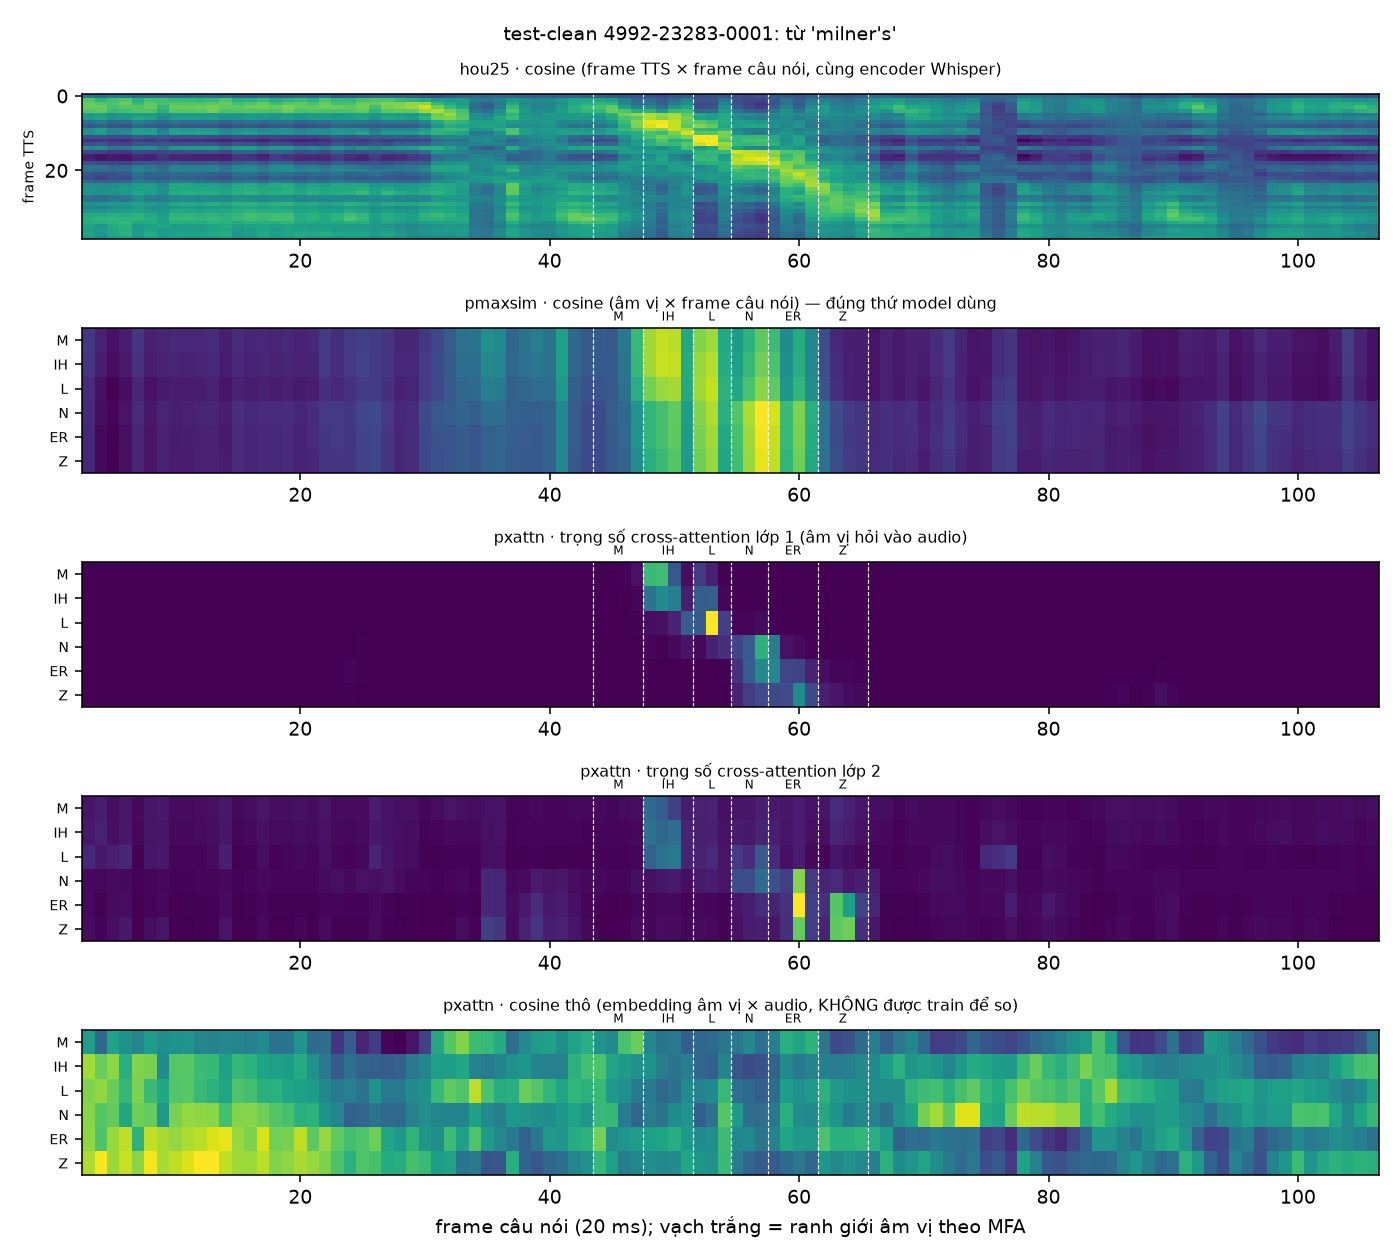
\includegraphics[width=\linewidth,height=0.80\textheight,keepaspectratio]{../../scorer/runs/2026-11-02/imgs/example_test-clean_0.png}
\end{column}
\end{columns}
\end{frame}

\begin{frame}{TN4 -- Hai phía khác loại (audio / âm vị) gặp nhau ở đâu?}
\centering
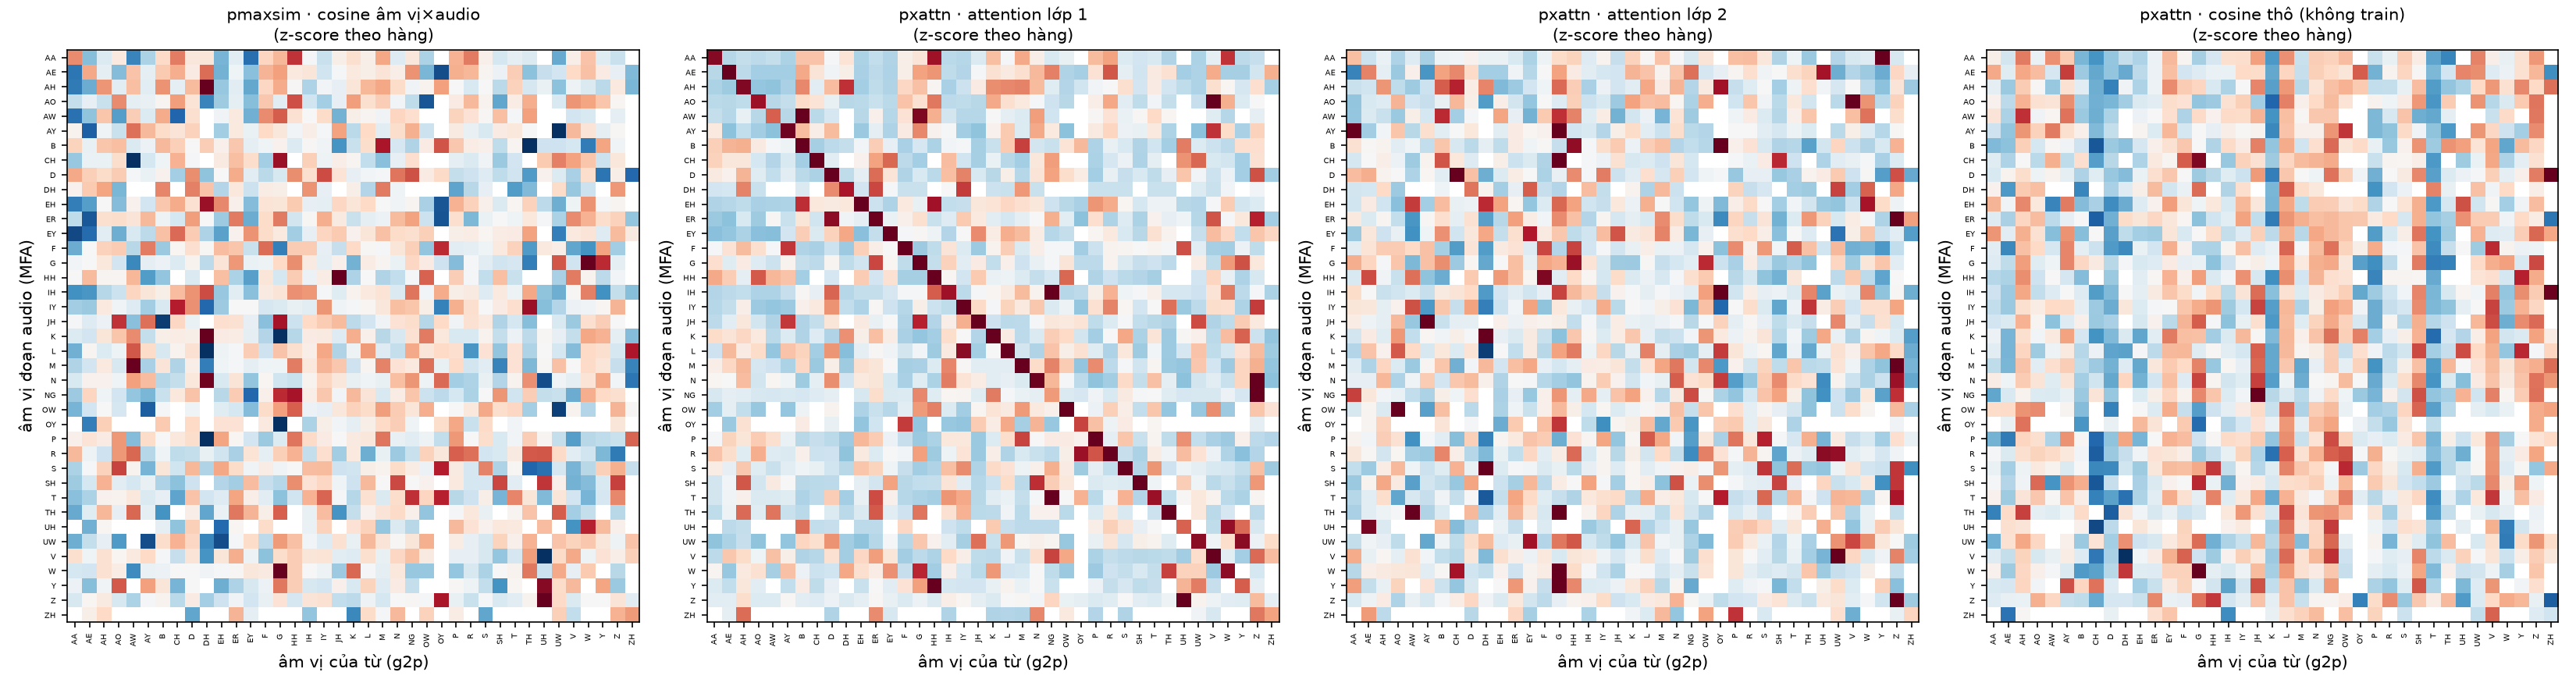
\includegraphics[width=\linewidth]{../../scorer/runs/2026-11-02/imgs/phone_matrix.png}\par
\vspace{0.15cm}\raggedright
\begin{columns}[T]
\begin{column}{0.48\textwidth}
\nbox{Ma trận 39 $\times$ 39: đường chéo lớn nhất ở \good{69\%} số hàng với attention lớp 1; pmaxsim 5\%; cosine thô 0\%.}
\end{column}
\begin{column}{0.48\textwidth}
\nbox{\textbf{Insight:} nhánh audio \textbf{không} bị ``âm vị hoá'' (probe: 66.7 / 58.6\%, ngang chiếu ngẫu nhiên). Hai phía gặp nhau trong \textbf{phép chiếu q/k của attention}.}
\end{column}
\end{columns}
\end{frame}

\begin{frame}{Các thí nghiệm còn lại}
\centering\scriptsize\setlength{\tabcolsep}{3pt}
\begin{tabular}{L{3.3cm}L{5.6cm}L{5.3cm}}
\toprule
Câu hỏi & Số chính & Insight\\
\midrule
Vị trí có thêm thông tin có/không? & AUC của $p$: 0.995--1.000; của đỉnh attention: 0.97 & Thời gian cho biết \textbf{ở đâu}, không thêm \textbf{có hay không}. Cần cả hai làm cổng. \\
\addlinespace
Vị trí qua prompt \src{Hoàng F13--F16, scorer Hou25} & oracle thứ tự nói $-$0.69 / $-$1.36; xếp cả 50 theo thời gian \bad{+0.42 / +0.58}; hybrid $p\geq0.3$: $-$0.17 / $-$0.41 & Qua prompt, vị trí giúp \textbf{ít}. Từ nhiễu không có thời gian thật nên xếp cả 50 từ thì hại. \\
\addlinespace
Giới tính giọng \src{biên bản 24/10} & 44 nữ / 29 nam (ước từ F0); mọi CI đều chứa 0, kể cả Hou25 dùng giọng TTS nữ & Không thấy ảnh hưởng. Giới tính chỉ là ước lượng. \\
\addlinespace
Câu nhiều từ hiếm \src{biên bản 24/10} & pxattn N100, câu $>$1 từ: 4.37 / 8.47; oracle 4.33 / 8.63 & Hưởng lợi đều; hỏng chỉ ở câu 0--1 từ hiếm khi prompt quá ngắn. \\
\bottomrule
\end{tabular}\par
\vspace{0.1cm}\raggedright
\nbox[block body alerted]{\textbf{Tổng kết:} với pxattn, phần scorer còn sửa được chỉ khoảng 2/10 điểm lỗi (test-other N2000). Lỗi lớn nhất là \hi{ASR viết sai dù từ đã có trong prompt}. Muốn đẩy xác suất mà không chèn sai thì cần biết \hi{có không} và \hi{ở đâu}.}
\end{frame}

% ------------------------------------------------------------------
\section{Chốt scorer}
\begin{frame}{Để dứt điểm scorer: còn 5 việc, S0 làm trước}
\centering\scriptsize\setlength{\tabcolsep}{4pt}
\begin{tabular}{cL{5.3cm}L{2.0cm}L{3.7cm}L{1.7cm}}
\toprule
\# & Việc & Chi phí & Tiêu chí xong & Trạng thái\\
\midrule
\textbf{S0} & \textbf{Âm vị--âm vị thật:} head CTC trên Whisper + căn chỉnh; thêm pxattn 1 lớp & GPU $\sim$10 h \src{ước lượng} & \#50 $\geq$ pxattn, H\#50 không tệ hơn, vị trí $\leq$0.05 s & \bad{mới}\\
S1 & So ghép cặp với Hou25 (Hoàng); phân rã lỗi của cả hai & CPU, nửa ngày & có CI; biết phần chênh từ đâu & \bad{chờ Hoàng}\\
S2 & \textbf{Temporal NMS}: hai ứng viên chồng thời gian thì giữ từ $p$ cao hơn & GPU $\sim$2 h & R\_H\#50 giảm $\geq$3; R\_B\#50 giảm $\leq$0.1 & chưa\\
S3 & Decode Whisper: top-50 sau NMS; prompt hybrid theo thời gian của pxattn & GPU $\sim$3 h & B-WER $\leq$ Hou25 trong CI & chưa\\
S4 & 3 seed kiến trúc được chọn & GPU 3 $\times$ $\sim$5 h & biết phương sai & chưa\\
\midrule
S5 & (chỉ khi S2 không đủ) negative khó theo khoảng cách âm vị & GPU $\sim$5 h & như S2 & dự phòng\\
\bottomrule
\end{tabular}\par
\vspace{0.25cm}\raggedright
\begin{columns}[T]
\begin{column}{0.48\textwidth}
\nbox{\textbf{Chốt sau S0:} đạt tiêu chí thì đổi, không đạt thì giữ pxattn. S2--S4 làm trên kiến trúc được chọn.}
\end{column}
\begin{column}{0.48\textwidth}
\nbox[block body alerted]{\textbf{Kỳ vọng:} theo TN2, NMS có thể giảm R\_H\#50, nhưng lợi B-WER trực tiếp nhỏ (thay = nhiễu chỉ 0.14 / 0.34).}
\end{column}
\end{columns}
\end{frame}

\section{Dùng vị trí}
\begin{frame}{Dùng vị trí: biasing lúc decode có cổng}
\begin{columns}[T]
\begin{column}{0.55\textwidth}
\footnotesize
\begin{itemize}\setlength{\itemsep}{3pt}
\item \textbf{Đầu ra mới} (không train lại): (từ, $p$, $t_{\text{đầu}}$, $t_{\text{cuối}}$, thời điểm từng âm vị). Với pxattn: đọc từ attention lớp 1, hiện model tính rồi bỏ đi.
\item \textbf{D0 -- mổ decode} \src{biên bản 24/10}: tại mỗi lỗi nghe giống, token đúng đứng hạng mấy, cách token được chọn bao xa \ra{} \hi{cần đẩy mạnh cỡ nào}.
\item \textbf{D1 -- boost có cổng} (Whisper): cộng điểm token của bias word \textbf{chỉ khi} $p\geq\tau$ \textbf{và} decoder đang nhìn vào $[t_{\text{đầu}}-\delta,\ t_{\text{cuối}}+\delta]$.
\item \textbf{D2 -- sang model khác}: nếu không đọc được ``đang ở frame nào'' thì dùng 2 lượt: hyp lần 1 có timestamp, chỉ boost trong cửa sổ.
\item \textbf{D3 -- đọc tài liệu logit}: shallow fusion, TCPGen, CB-Whisper, BPB, PTC-Bias. \bad{Mới biết tên, chưa đọc toàn văn.}
\end{itemize}
\end{column}
\begin{column}{0.42\textwidth}
\centering\scriptsize\setlength{\tabcolsep}{3pt}
\begin{tabular}{lcc}
\toprule
Arm D1 & cổng $p$ & cổng $t$\\
\midrule
boost trần & -- & --\\
chỉ $p$ & có & --\\
chỉ thời gian & -- & có\\
\textbf{cả hai} & \good{có} & \good{có}\\
\bottomrule
\end{tabular}\par
\vspace{0.2cm}\raggedright
\nbox{\textbf{Đo:} B-WER, U-WER, và \hi{số lần chèn trên \texttt{missing\_N2000}}: list không có từ đúng nên mọi lần chèn đều sai. Trả lời câu ``không chèn khi audio không có'' \src{biên bản 1/11}.}
\vspace{0.1cm}
\nbox[block body alerted]{\textbf{Đóng góp (ta diễn giải):} cổng dùng cho nhiều kiểu ASR, không cần train lại ASR. \bad{Chưa chạy.}}
\end{column}
\end{columns}
\end{frame}

\section{SpeechLLM}
\begin{frame}{Chọn SpeechLLM để thực nghiệm}
\relax{\small\textbf{Tiêu chí:} (1) open weight, can thiệp được logit từng bước; (2) \textbf{các họ kiến trúc khác nhau}, để trả lời ``cách nào tổng quát''; (3) vừa 1 card 24 GB.}\par\vspace{0.2cm}
\centering\scriptsize\setlength{\tabcolsep}{4pt}
\begin{tabular}{L{2.9cm}L{3.4cm}L{3.5cm}L{3.9cm}}
\toprule
Họ & Model & Vai trò & Biết ``đang ở đâu'' bằng gì\\
\midrule
encoder--decoder & \textbf{Whisper-large-v3-turbo} & tái hiện Hou25; làm D0, D1 trước & cross-attention (như word timestamp)\\
audio encoder + LLM & \textbf{Qwen3-ASR-1.7B} & backbone chính; so với PTC-Bias & \bad{chưa kiểm}: attention vào token audio, hoặc 2 lượt\\
audio encoder + LLM lớn hơn & ứng viên: Qwen2-Audio, Phi-4-multimodal, Voxtral & kiểm tính tổng quát & \bad{chưa kiểm}\\
CTC / transducer (tuỳ chọn) & ứng viên: NeMo Parakeet & cổng khi không có LLM & thời gian có sẵn theo frame\\
\bottomrule
\end{tabular}\par
\vspace{0.3cm}\raggedright
\nbox{\textbf{Đề xuất:} Whisper + Qwen3-ASR là bắt buộc; thêm 1 model thứ 3 nếu kịp. Các ứng viên chưa kiểm license, bộ nhớ và cách đưa context; sẽ kiểm trước khi chọn.}
\end{frame}

\section{Kế hoạch}
\begin{frame}{Lịch tới hạn nộp 09/02/2027 (còn khoảng 14 tuần)}
\centering\footnotesize\setlength{\tabcolsep}{5pt}
\begin{tabular}{clL{5.2cm}L{5.0cm}}
\toprule
Tuần & Đến & Việc & Kết quả\\
\midrule
1--2 & 17/11 & S0 rồi S1--S4: chọn kiến trúc, chốt scorer & bảng A--D đủ CI; nháp chương scorer\\
3--4 & 01/12 & D0 trên Whisper + Qwen; đọc tài liệu logit & biết cần boost bao nhiêu; chốt thiết kế D1\\
5--7 & 22/12 & D1 trên Whisper: 4 arm, N100/N2000, \texttt{missing} & bảng chính: B-WER giảm, chèn sai không tăng\\
8--9 & 05/01 & D2: Qwen3-ASR (+ model 3 nếu kịp) & cùng bảng trên SpeechLLM\\
10 & 12/01 & Tập ngoài LibriSpeech (ConEC / Earnings) & kiểm domain thật\\
11--14 & 09/02 & Ablation, viết paper, nộp & --\\
\bottomrule
\end{tabular}\par
\vspace{0.3cm}\raggedright
\nbox[block body alerted]{\textbf{Rủi ro:} (1) D1 không thắng prompt hybrid \ra{} paper dừng ở scorer + NMS + prompt. (2) GPU dùng chung, lần gần nhất cả 4 card đều bận \ra{} cần lịch card. (3) Chưa có file Hoàng \ra{} S1 trễ, nhưng không chặn S2--S4. (4) S0 thắng \ra{} phải làm lại Bảng A, B, nên tuần 1--2 có thể trễ.}
\end{frame}

\begin{frame}{Cần thầy quyết}
\begin{enumerate}\setlength{\itemsep}{7pt}
\item \textbf{Định vị đóng góp:} ``gần bằng Hou25 nhưng không cần TTS, có ngưỡng, có vị trí'', thay cho ``thắng Hou25''?
\item \textbf{Chạy S0 (âm vị--âm vị) trước khi chốt}, rồi mới chuyển sang decode (D0--D2)?
\item \textbf{Paper chính} là scorer + cổng thời gian lúc decode, hay chỉ scorer (an toàn hơn, ít mới hơn)?
\item \textbf{Model thứ 3:} có cần không, ưu tiên model nào?
\item \textbf{GPU:} xin card cố định cho tuần 1--2 (khoảng 30 h \src{ước lượng}, chủ yếu để train S0 và S4).
\end{enumerate}
\end{frame}

\end{document}
